\chapter{Darstellung der Ergebnisse}
In diesem Kapitel setzen Sie den zuvor ausgewählten Lösungsweg systematisch um. Sie beschreiben die Umsetzung und dokumentieren die Ergebnisse zu denen Sie gekommen sind. Es ist denkbar, dass das Ergebnis lautet: "`Dieser Lösungsweg schien laut Kapitel \ref{cha:Loesungswege} vielversprechend, hat jedoch das Problem nicht gelöst."' Diese Erkenntnisse sind jedoch auch wichtig und richtig und sollten im nachfolgenden Kapitel diskutiert werden.

\section{Versuchsdurchführung}
In diesem Abschnitt beschreiten Sie Ihren Lösungsweg. Dokumentieren Sie alles, was nötig ist, um Ihre Ergebnisse zu reproduzieren.

\section{Versuchsauswertung}
Die Versuchsauswertung erfolgt anhand der gemessenen Daten in Form von Messwerttabellen, Diagrammen und Abbildungen.
Tabellen besitzen immer eine Kopfzeile und eine Führungsspalte.
Die Kopfzeile enthält die Oberbegriffe zu den Spalten und die Führungsspalte Oberbegriffe zu den Zeilen.
Die Begriffe in der Kopfzeile und in der Führungsspalte sollen in sich konsistent und logisch gleichwertig sein \cite[S.~51]{Hering2009}.
Innerhalb der wissenschaftlichen Arbeit sollte eine gleich bleibende Tabellengestaltung beibehalten werden.
Die Eintragungen in den Zellen einer Tabelle können Zahlen, Wörter, Skizzen oder Kombinationen aus diesen Elementen sein.
Für die Eintragungen gelten die normalen Regeln der Groß- und Kleinschreibung, d.\,h. vor allem Adjektive beginnen mit kleinen Buchstaben.
Texte werden innerhalb der Zellen linksbündig ausgerichtet, da eine zentrierte Textausrichtung ein oft zu unruhiges Layout ergibt.
Die Tabellennummern können durch den ganzen Bericht hindurch fortlaufend hochgezählt werden wie es in dieser Ausarbeitung gehandhabt wurde.
Sie können jedoch auch zusammengesetzt werden aus der Kapitelnummer und der innerhalb eines Kapitels fortlaufend hoch gezählten Tabellennummer \cite[S.~54~ff.]{Hering2009}.

In der nachfolgenden Tabelle \ref{tbl:Laplace} wird veranschaulicht wie Tabellen in den Bereicht eingebunden werden\footnote{Auf jede im Text angeordnete Tabelle sollte im Text mindestens einmal hingewiesen werden (vgl. \cite{Hering2009}, S. 58).}.
In diesem Beispiel werden die Tabellennummern durch den Bericht hindurch fortlaufend hochgezählt.
Die Tabellen\textbf{überschrift} mit Nummerierung und Benennung steht im Gegensatz zu Grafiken zentriert oberhalb der Tabelle.
Grafische Abbildungen wie Fotos oder Screenshots werden üblicherweise in unveränderter Form mit Quellenverweis übernommen.
Tabellen sollten jedoch neu erstellt werden, wobei die Inhalte aus der fremden Quelle übernommen werden, damit durchgängig die gleiche Schriftart und -größe verwendet wird \cite[S.~113]{Balz2008}.

\begin{table*}[h]
	\centering
	\caption{Laplace Transformation, Quelle: \cite{Kiencke2001}}
	\label{tbl:Laplace}
		\begin{tabular}[t]{|l|l|l|}
		\hline
		allg. Eigenschaft / Operation & Zeitfunktion $f(t)$ & Bildfunktion $F(s)$\\ \hline
		Linearität & $a_{1}f_{1}(t)+a_{2}f_{2}(t)$ & $a_{1}F_{1}(s)+a_{2}Ff_{2}(s)$\\ \hline
		Ähnlichkeitssatz & $f(at)$ & $\frac{1}{a}F(\frac{s}{a})$ für $a>0$\\ \hline
		Verschiebung im Originalbereich & $f(t-a)$ & $e^{-as}F(s)$\\ \hline
		Verschiebung im Bildbereich & $e^{-at}\cdot{f(t)}$ & $F(s+a)$ mit $(a\in{C})$\\ \hline
		Sinus-Multiplikation & $sin(at)\cdot{f(t)}$ & $\frac{1}{2i}(F(s-ia)-F(s+ia))$\\ \hline
		Cosinus-Multiplikation & $cos(at)\cdot{f(t)}$ & $\frac{1}{2}(F(s-ia)+F(s+ia))$\\ \hline
		\end{tabular}
\end{table*}

\noindent
Bei kleineren Tabellen wird bewirkt, dass Informationen sehr systematisch, übersichtlich und strukturiert dargestellt werden.
Im Gegensatz dazu wirken größere Tabellen oft unübersichtlich.
Es fällt dem Leser einer großen Zahlen-Tabelle meist schwer, Verhältnisse von Zahlen abzuschätzen und Größen miteinander zu vergeleichen.
Deshalb sollte man große Zahlen-Tabellen in Diagrammform visualisieren.
Trotzdem müssen die Berechnungen, statistischen Auswertungen und Versuchsergebnisse mit exakten Zahlen belegt werden.
Die umfangreichen Zahlen-Tabellen können im Anhang untergebracht werden.
Im Text erscheinen aussagekräftige Visualisierungen und die zugehörigen Tabellen werden mit einem Verweis auf den Anhang referenziert \cite[S.~52]{Hering2009}.

Bei Diagrammen gilt als Grundprinzip, dass eindeutige Beschriftungen von Achsen, Säulen, Sektoren usw. erforderlich sind.
Graphen mit farbigen Kurven sollten immer eine Legende besitzen.
Oft kann die Verständlichkeit eines Diagramms auch dadurch gesteigert werden, dass die Aussage als Titel bzw. Beschriftung direkt über oder neben dem Diagramm erscheint. 
Ein Beispiel, wie Diagramm und Titel bzw. Beschriftung zusammenwirken können, zeigt Abbildung 2 \cite[S.~84~f.]{Hering2009}.

\begin{figure}[h]
	\centering
		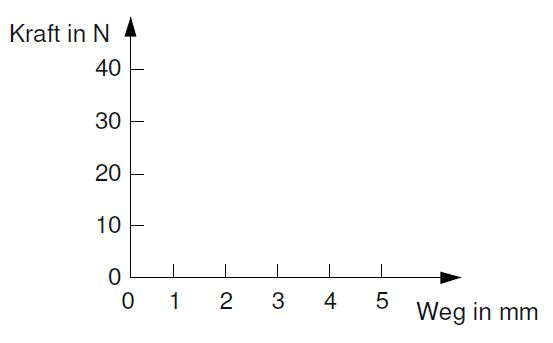
\includegraphics[width=0.6\textwidth]{Diagramm1.jpg}\\
			\caption{Beispielhaftes Diagramm zur Verdeutlichung der Anordnung nach \cite{Hering2009}}
		\label{fig:Diagramm1}
\end{figure}

\noindent
Alle Diagramme und Bilder erhalten eine Bildunterschrift mit Bildnummer.
Dabei sollte die Anordnung und Formatierung der Bildunterschriften einheitlich sein.
Die Achsen müssen genau beschriftet werden mit Achsenbezeichnung (als Text oder Formelbuchstabe) und zugehöriger Maßeinheit, Maßzahlen und Pfeilen an den Achsenenden (die Pfeile zeigen nach oben und rechts).
Eine horizontale Text-Angabe sowie die waagerechte Beschriftung der Achsen ist unbedingt vorzuziehen, weil die Grafik so nicht gedreht werden muss.
Wenn ein Diagramm zum Ablesen von Zahlen dient, dann ist die Verwendung von Netzlinien vorteilhaft.
Solbald in einem Diagramm mehrere Kurven eingezeichnet werden sollen, müssen die Kurven eindeutig zu unterscheiden sein.
Dafür können verschiedene Farben, Linienarten und Messpunktsymbole verwendet werden \cite[S.~85~ff.]{Hering2009}.